\documentclass[a4paper]{article}
\usepackage[a4paper,top=2cm,bottom=2.5cm,left=1.5cm,right=1.5cm,marginparwidth=1.75cm]{geometry}
%% Language and font encodings
\usepackage[english]{babel}
\usepackage[utf8x]{inputenc}
\usepackage{listings}
\usepackage{hyperref}
\usepackage{float}
%% Sets page size and margins
\usepackage{setspace}
\usepackage{graphicx,float}
\renewcommand{\baselinestretch}{1} 
\usepackage{float}
%% Useful packages
\usepackage{amsmath}
\usepackage[colorinlistoftodos]{todonotes}
\usepackage[colorlinks=true, allcolors=blue]{hyperref}
\usepackage{listings}
\usepackage{url}
\usepackage{xcolor}
\graphicspath{ {./images/} }
% \DeclareGraphicsExtensions{.pdf,.jpg,.png}

%% defined colors
\definecolor{Blue}{rgb}{0,0,0.5}
\definecolor{Green}{rgb}{0,0.75,0.0}
\definecolor{LightGray}{rgb}{0.6,0.6,0.6}
\definecolor{DarkGray}{rgb}{0.3,0.3,0.3}

\title{COP290: Assignment - 1(3)}
\author{
Himanshu Gaurav Singh \\ 
2019CS10358 
\\ \\
Abhinav Jain \\
2019CS10322 \\  }
%date{February  1, 2021 }%
\begin{document}
\maketitle
\begin{center} \textbf{ \Large Trade-off analysis for software design choices} 
\end{center}
\section*{Abstract}
%\subsection*{Input Format}%
% \paragraph{}
\begin{itemize}
\item We analyse the runtime vs utility trade-off between various implementation approaches to the problem of determining queue and dynamic density on a road using \textit{OpenCV} library functions.
\item The baseline for the analysis is the output of the queue and dynamic density functions submitted in Assignment-1 Subtask 2. 
\item The parameters over which the analysis has been done are : 
\begin{itemize}
    \item Number of frames skipped.
    \item Resolution of the image.
    \item Spatial multi-threading.
    \item Temporal multi-threading.
\end{itemize} 
\end{itemize}    
\section *{Metrics}
\begin{itemize}
    \item The utility metric is the root-mean-squared-error from the baseline output(distance from baseline output in the L-2 norm). More the error, less the utility. 
    \item The runtime metric is the time taken to run the whole program on my laptop(a quad-core MacOS machine).
    \item For the analysis of concurrent methods in Part-3 and Part-4, CPU utilisation is also used as a metric.
\end{itemize}
\section*{Method-1 : Sub-Sampling Frames}
\subsection*{Methodology}
The baseline code sub-samples one among every three frames. The skipping count (say \textit{x}) was varied over 3,6,9,12,15,18,21 to get the outputs and then compared with the baseline results. 
\subsection*{Results}
The following plot describes the obtained results.
\begin{figure}[H]
    \centering
    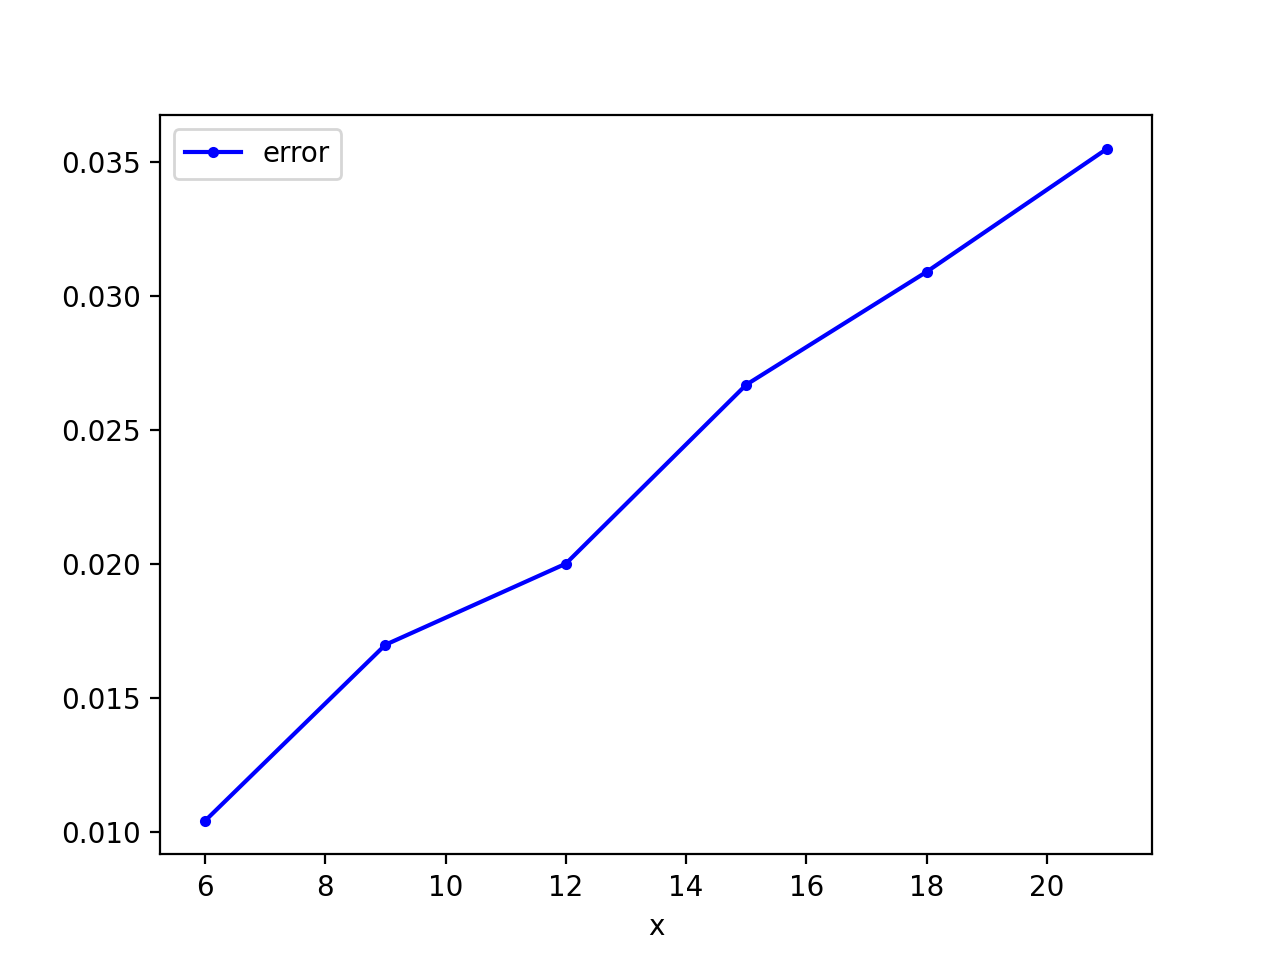
\includegraphics[width=0.5\linewidth]{method-1-error.png}
    \caption{Error v/s x}
    \label{fig:method-1-error.png}
\end{figure}
\begin{figure}[H]
    \centering
    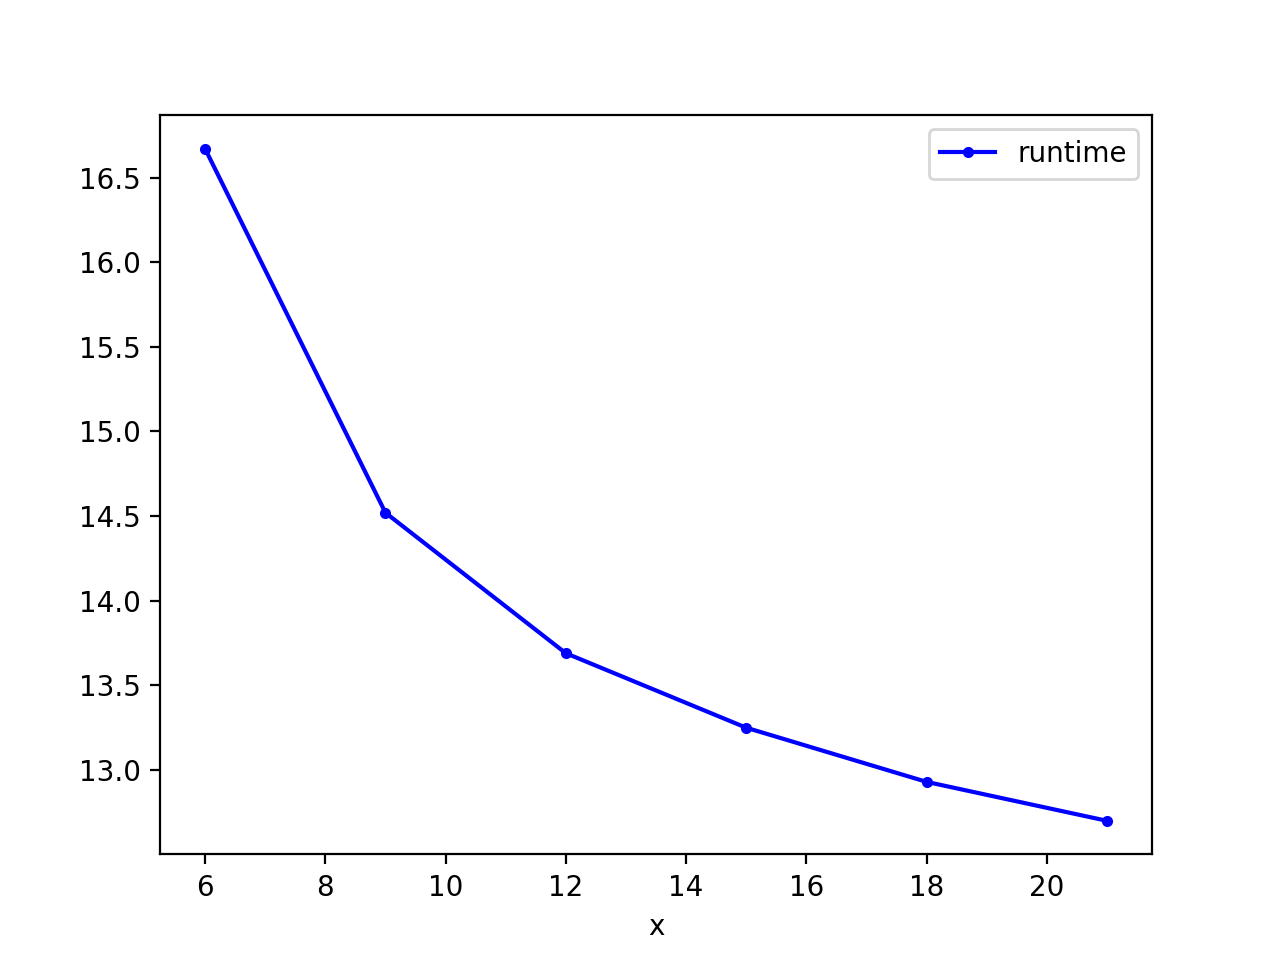
\includegraphics[width=0.5\linewidth]{method-1-runtime.png}
    \caption{Runtime v/s x}
    \label{fig:method-1-runtime.png}
\end{figure}
\begin{figure}[H]
    \centering
    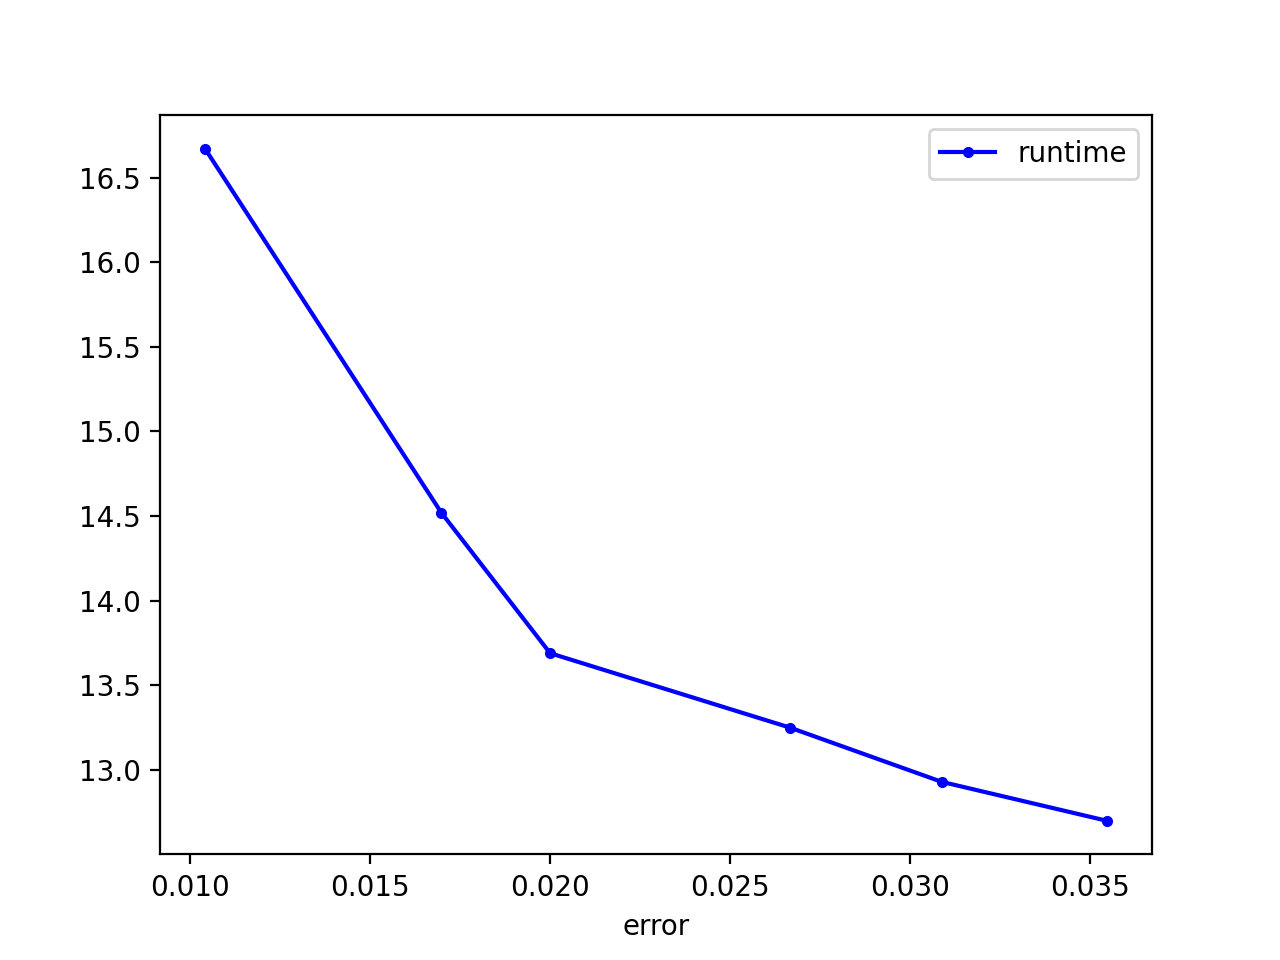
\includegraphics[width=0.5\linewidth]{method-1.png}
    \caption{Error v/s Runtime}
    \label{fig:method-1.png}
\end{figure}

%plot of runtime vs utility here 
\subsection*{Observation \& Explanation}
An increase in the error and a decrease in runtime is observed on increasing \textit{x}. The runtime decreases because less number of frames are processed as the skipping count increases. The error increases because we attempt to approximate the benchmark with a set of lesser number of frames as we increase \textit{x}.
\section*{Method-2 :  Modification of frame resolution }
\subsection*{Methodology}
The resolution of the frames are decreased as soon as they are captured before processing them. It is made sure that the row-column dimension ratio of the modified frame are same as that of the original frame.
\subsection*{Results}
The following plot describes the obtained results.
\begin{figure}[H]
    \centering
    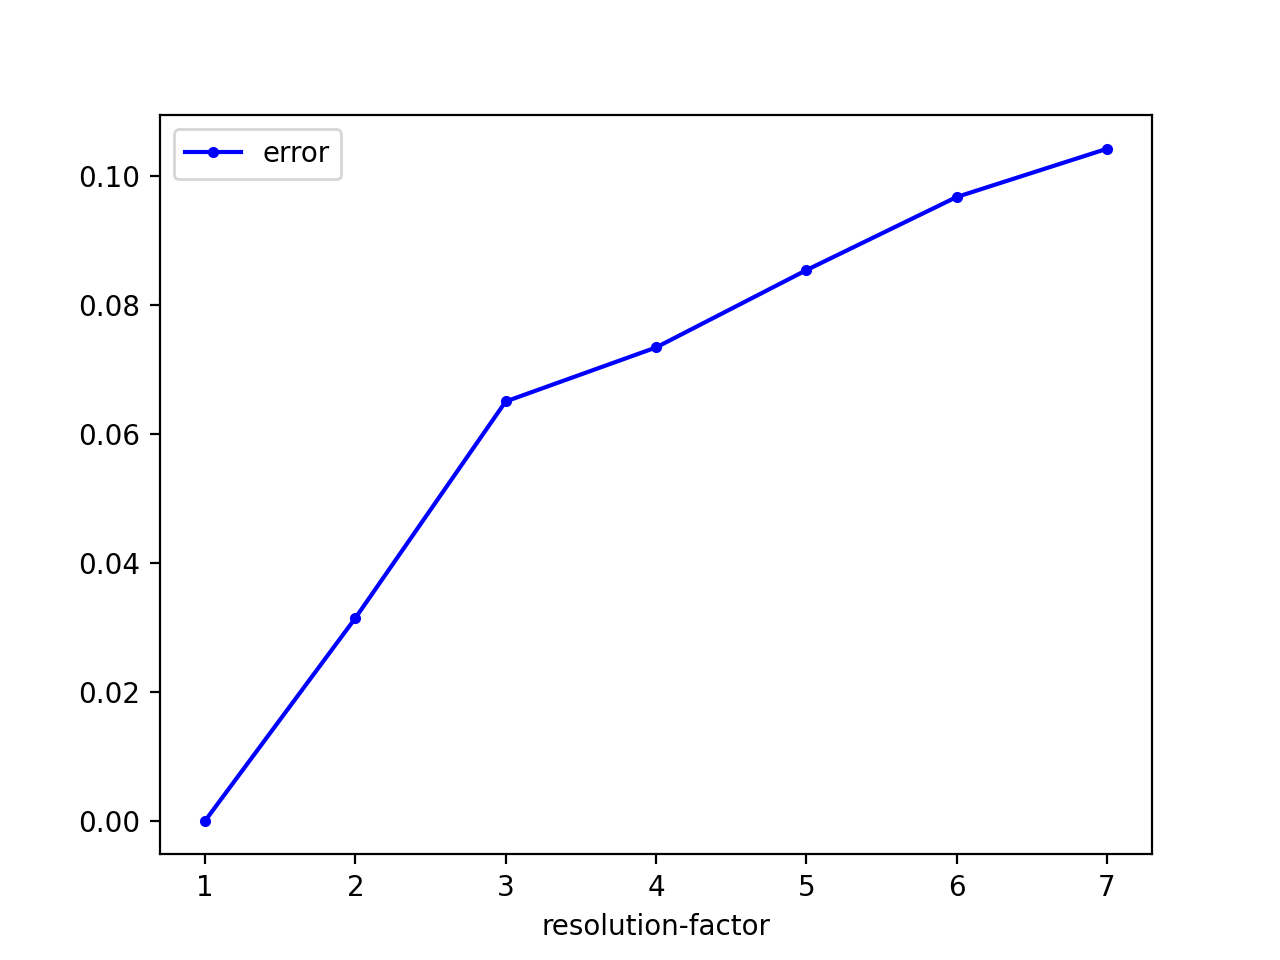
\includegraphics[width=0.5\linewidth]{resolution-error.png}
    \caption{Error v/s Resolution-factor}
    \label{fig:spatial-thread-error.png}
\end{figure}
\begin{figure}[H]
    \centering
    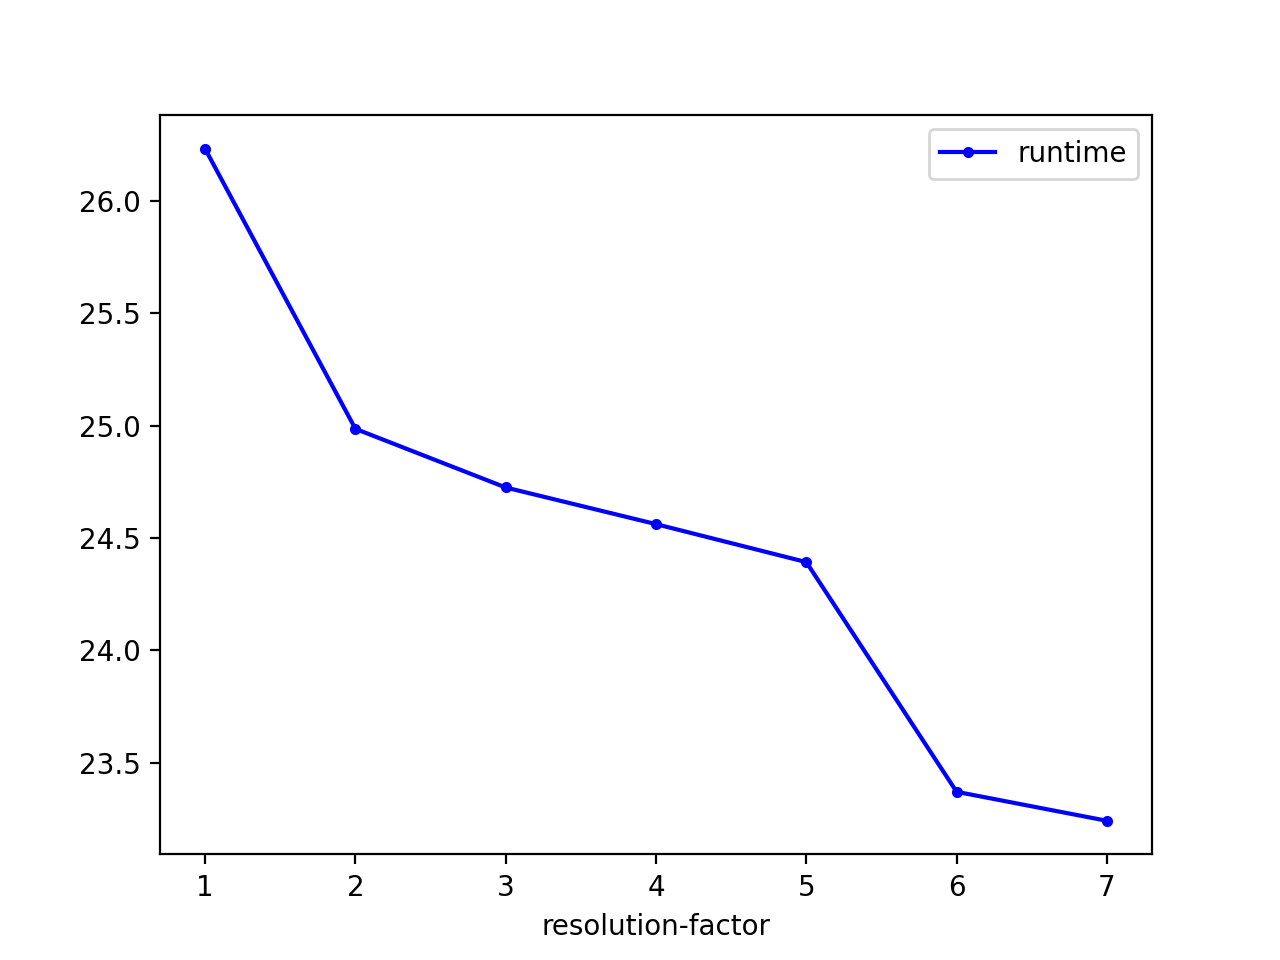
\includegraphics[width=0.5\linewidth]{runtime-resolution.png}
    \caption{Runtime v/s Resolution-factor}
    \label{fig:spatial-thread-error.png}
\end{figure}
\begin{figure}[H]
    \centering
    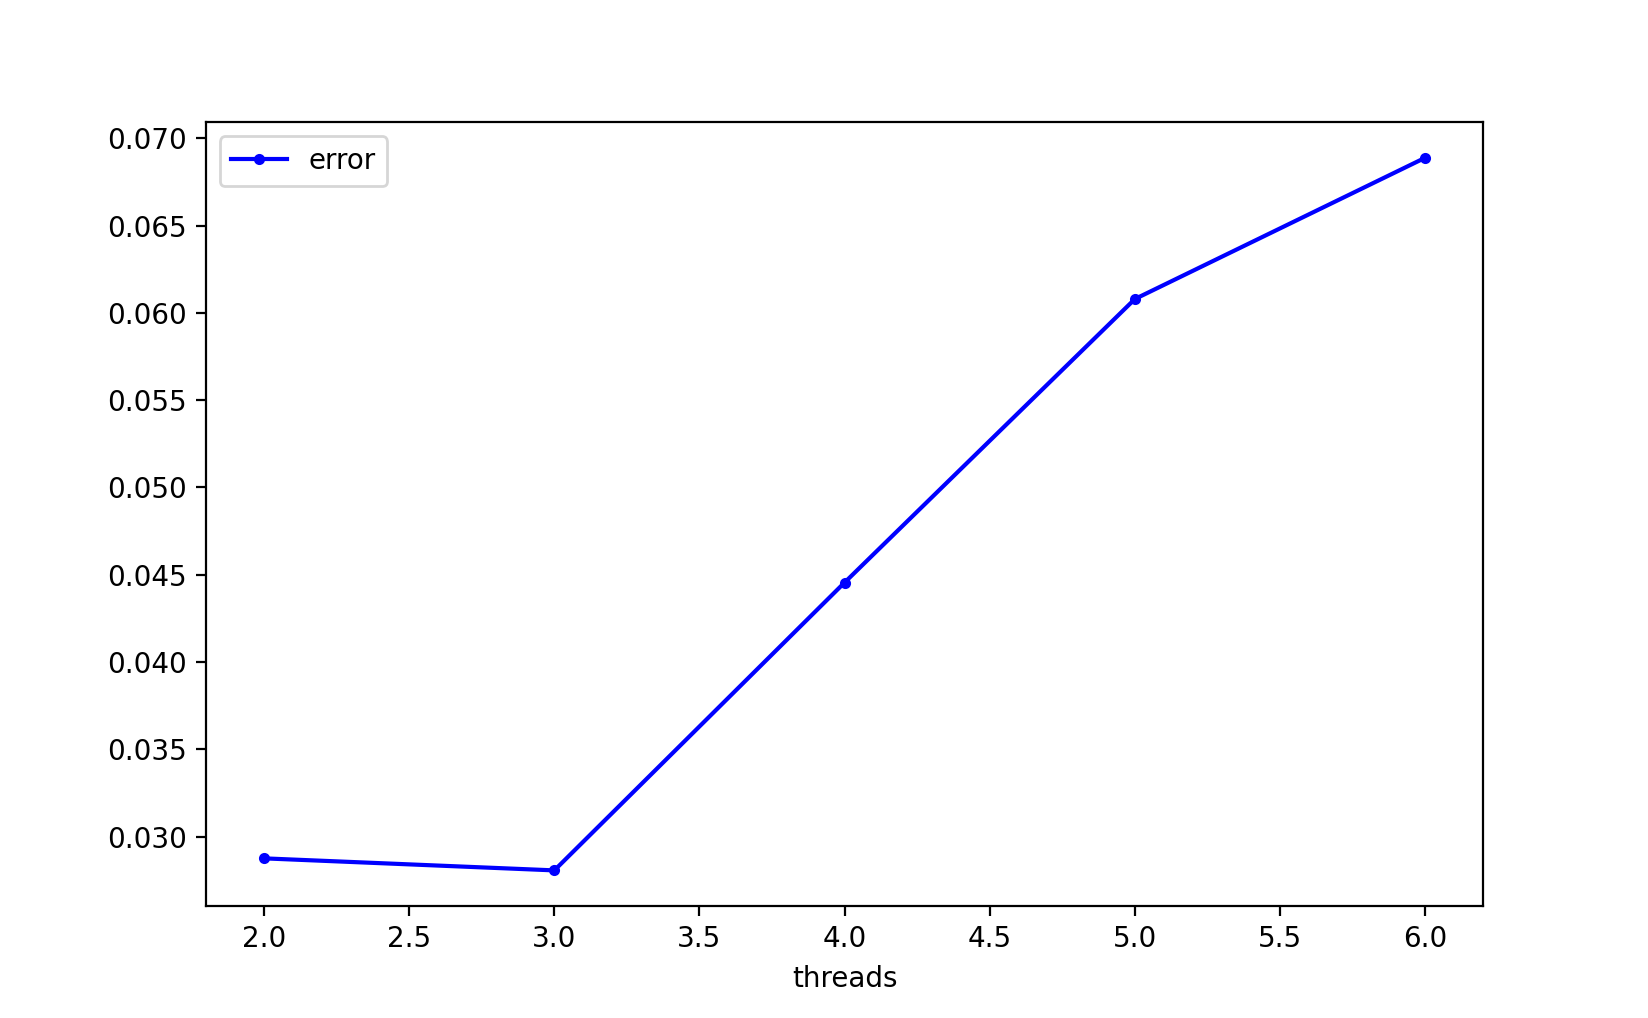
\includegraphics[width=0.5\linewidth]{spatial-thread-error.png}
    \caption{Error v/s Runtime}
    \label{fig:spatial-thread-error.png}
\end{figure}
%plot of runtime vs utility here 
\subsection*{Observation \& Explanation}
An increase in the error and a decrease in runtime is observed on decreasing resolution. The runtime decreases because we process a smaller image matrix per frame as compared to the benchmark. The error increases because we attempt to approximate every frame with a smaller, averaged-out matrix as we decrease resolution.
\section*{Method-3 : Spatial Multi-threading}
\subsection*{Methodology}
\begin{itemize}
    \item After capturing, each frame is divided into horizontal stripes same in number as the number of threads and then each stripe is passed-on to a separate thread. 
    \item We tried to provide different divisions of the original frame depending upon the number of threads(dividing the original into four squares) but observed no significant advantage. Hence, we decided to stick to a generic implementation for the sake of uniformity. 
\end{itemize}
\subsection*{Results}
The following plot describes the obtained results.
\begin{figure}[H]
    \centering
    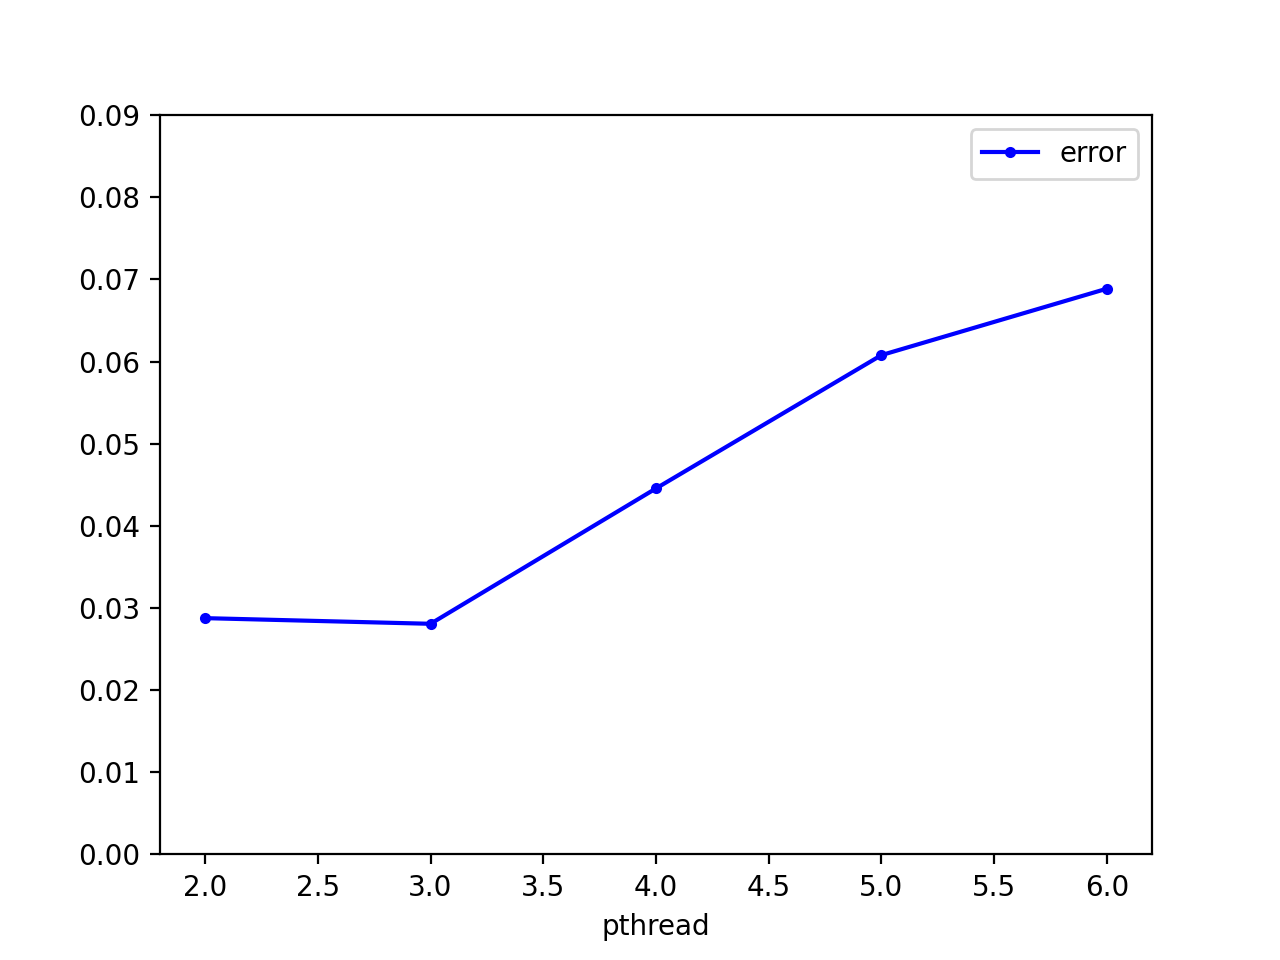
\includegraphics[width=0.5\linewidth]{spatial-pthreads-error.png}
    \caption{Error v/s Number of threads}
    \label{fig:spatial-pthreads-error.png}
\end{figure}
\begin{figure}[H]
    \centering
    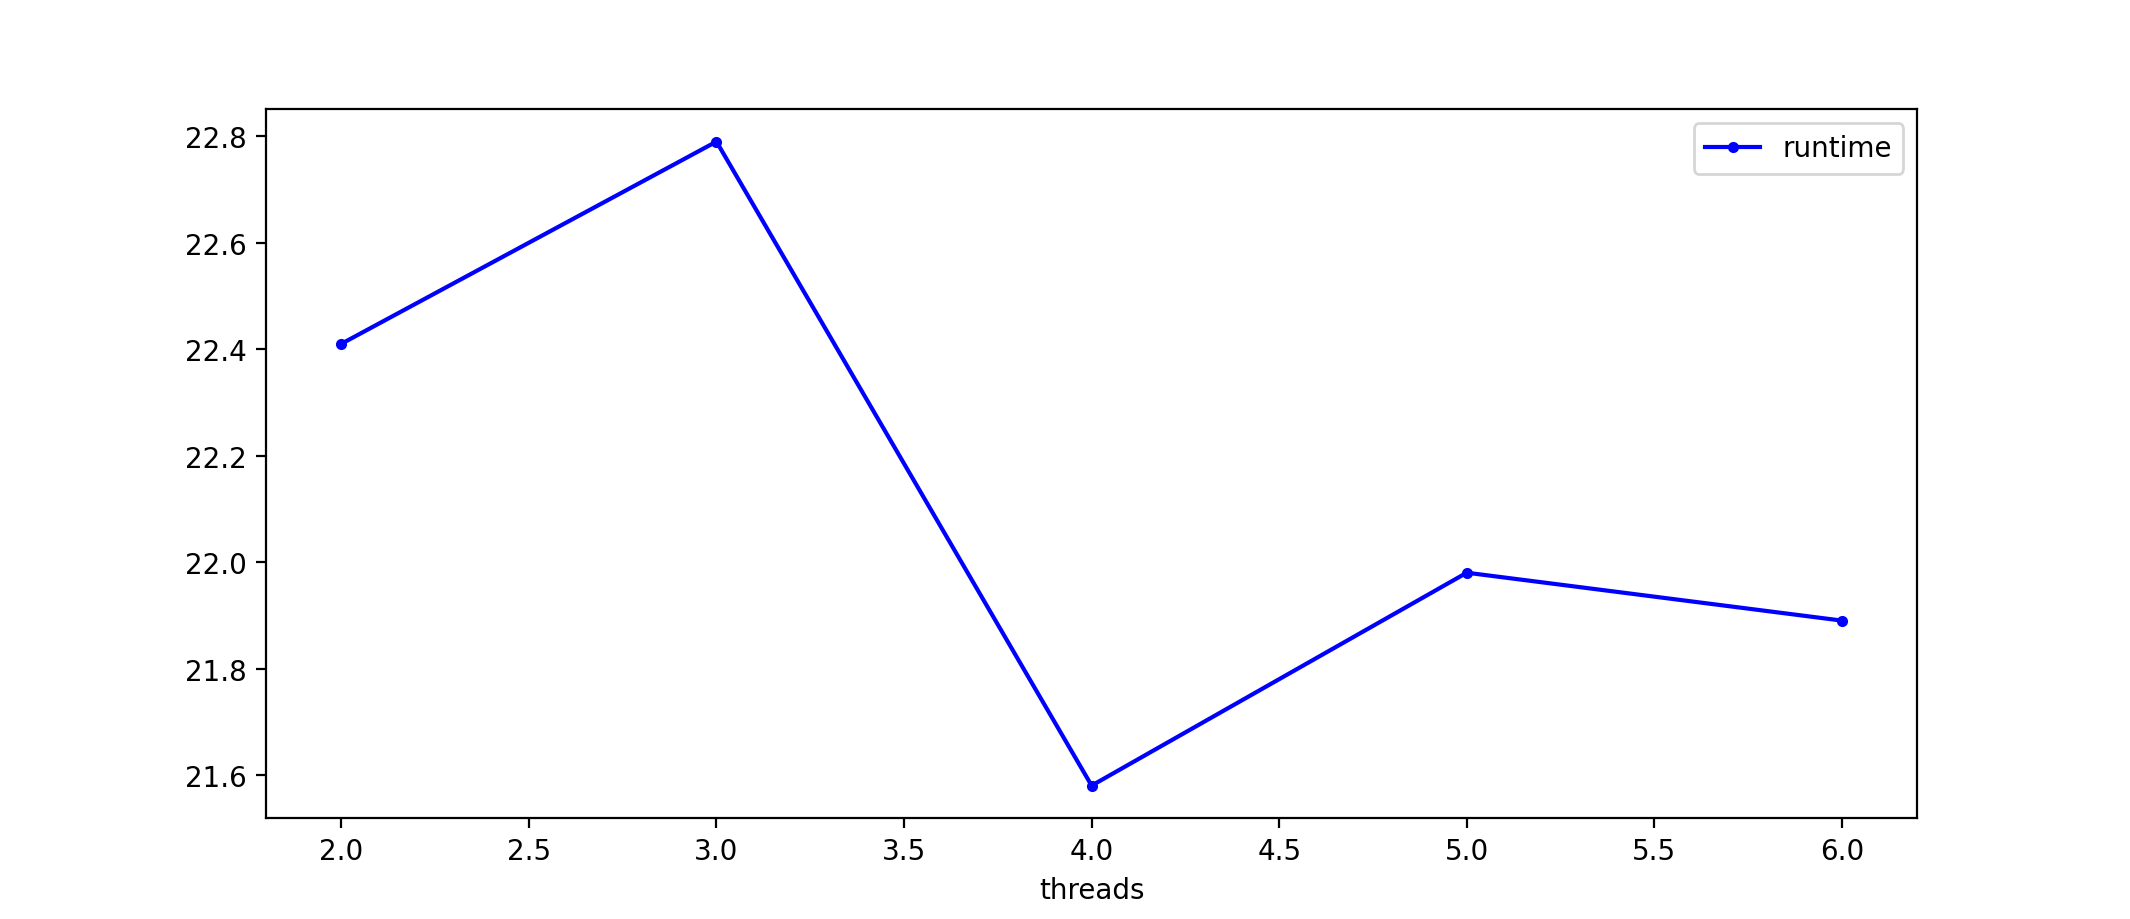
\includegraphics[width=0.5\linewidth]{spatial-thread-runtime.png}
    \caption{Runtime v/s Number of threads}
    \label{fig:spatial-thread-runtime.png}
\end{figure}
\begin{figure}[H]
    \centering
    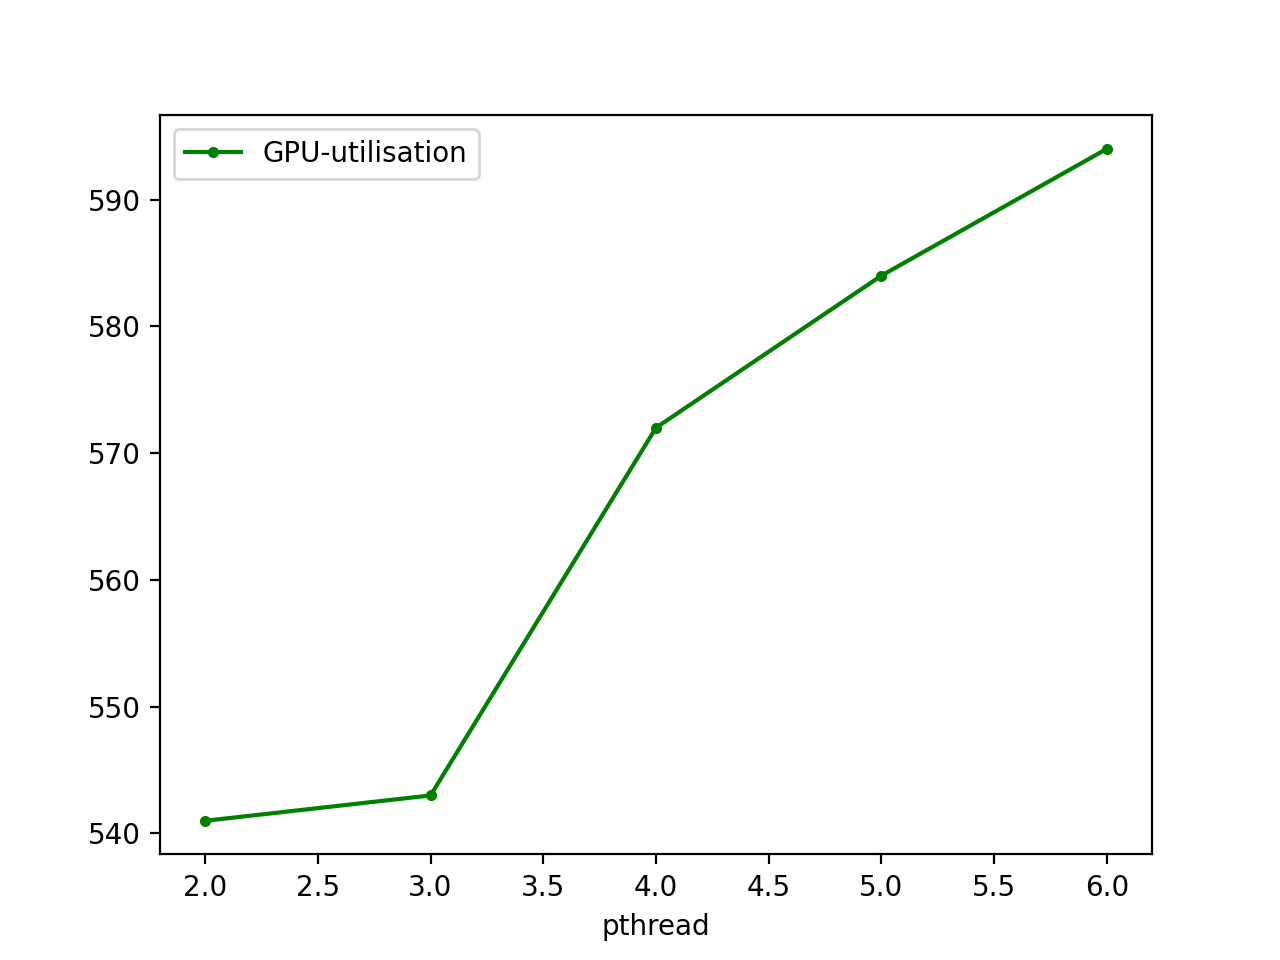
\includegraphics[width=0.5\linewidth]{spatial-pthreads-GPU-utilisation.png}
    \caption{CPU usage v/s Number of threads}
    \label{fig:spatial-pthreads-GPU-utilisation.png}
\end{figure}
%plot of runtime vs utility here 
\subsection*{Observation \& Explanation}
\begin{itemize}
    \item An increase in the error is observed with increase in number of threads. By dividing the original frame into several frames, we create several "edges/boundaries" in the image. In the image processing involved in dense optical flow, the edge pixels are not processed as properly as others. Hence the error increases as the number of threads in spatially concurrent sparse optical flow increases. 
    \item The plot shows no observable trend between runtime as the number of threads increases. \item A likely explanation that we came up was that the frame processing required for queue density is not large enough to result in a noticeable runtime gain on parallelization.\textbf{In the case of queue density estimation, the bottleneck for runtime is the time needed for capturing the frames and not the subsequent image processing}. Any minuscule gains by parallelizing are nullified by the overhead required for creating threads. No observable indications show up on CPU utilisation either.
    \item To validate our hypothesis, we ran code that just went through all the frames with the same speed as the baseline code and indeed, it's runtime was sufficiently close to the baseline runtime, hence, strengthening our hypothesis.
    \item As the number of threads increases, the average CPU usage increases since more of the resources get allocated to the running program.
\end{itemize}`
\section*{Method-4 : Temporal Multi-threading}
\subsection*{Methodology}
\begin{itemize}
    \item After capturing, every \textit{i}-th frame is alloted to the \textit{i}-th pthread.  The return values from threads are sorted on the basis of timestamps attached to the frame.
\end{itemize}
\subsection*{Results}
The following plot describes the obtained results.
\begin{figure}[H]
    \centering
    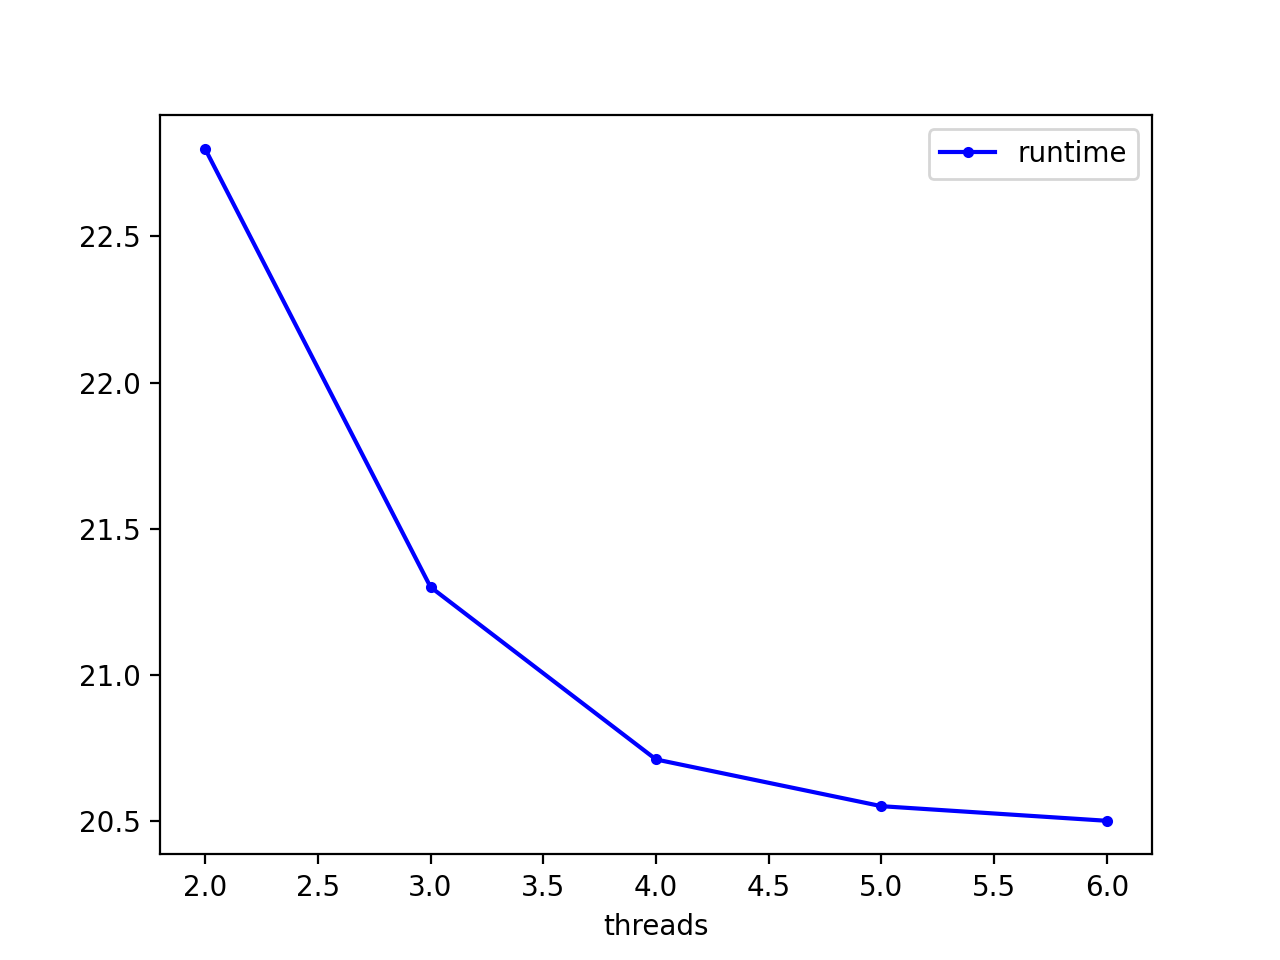
\includegraphics[width=0.5\linewidth]{temporal-threads-runtime.png}
    \caption{Runtime v/s Number of threads}
    \label{fig:spatial-threads-runtime.png}
\end{figure}
\begin{figure}[H]
    \centering
    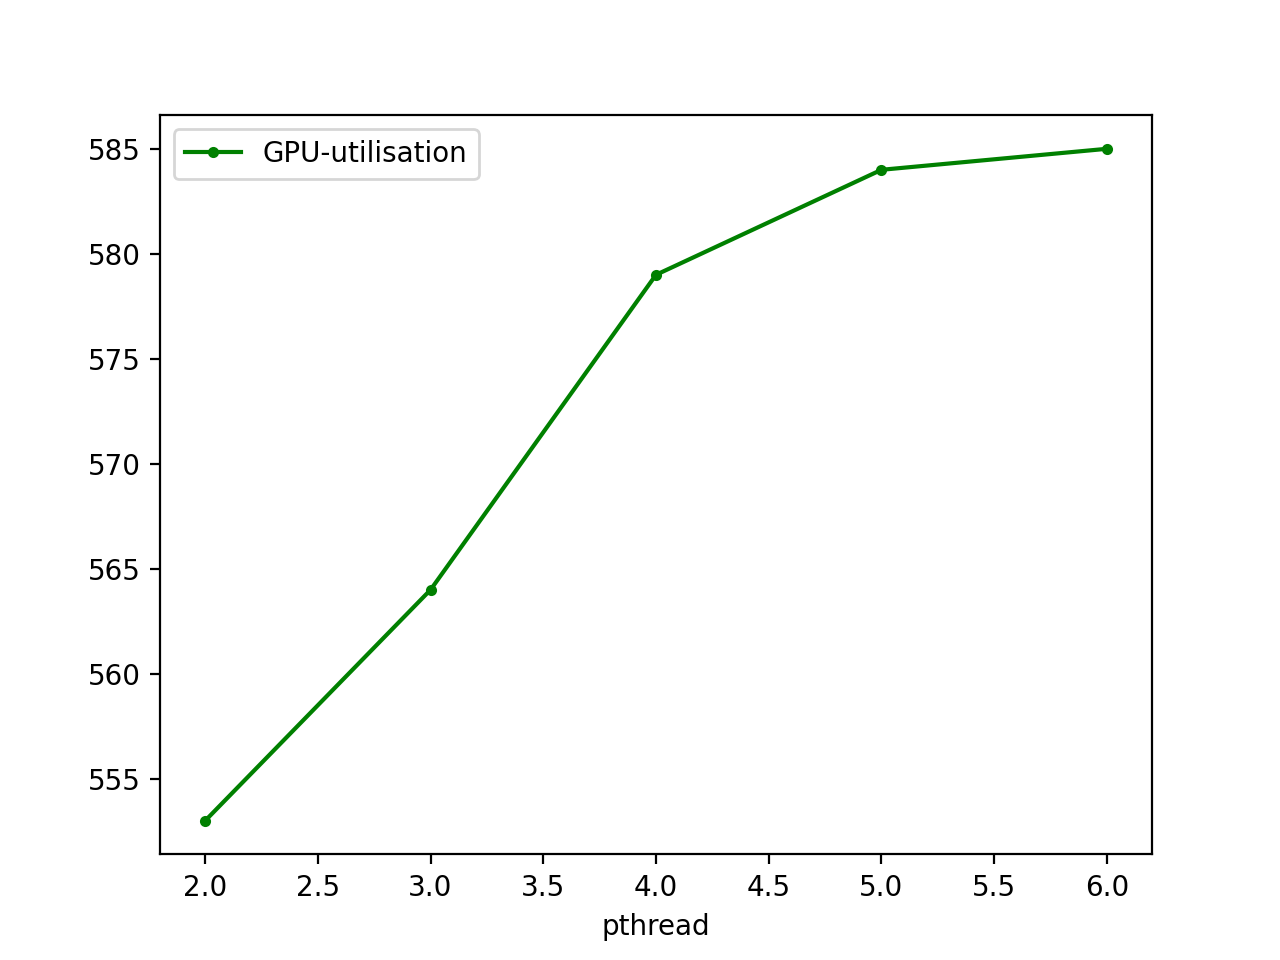
\includegraphics[width=0.5\linewidth]{temporal-thread-GPU-utilisation.png}
    \caption{CPU usage v/s Number of threads}
    \label{fig:temporal-thread-GPU-utilisation.pn}
\end{figure}
%plot of runtime vs utility here 
\subsection*{Observation \& Explanation}
\begin{itemize}
    \item The error in temporal concurrency is negligible in comparison to that in spatial concurrency. This is reasonable since the frames are processed exactly similar to the way in the non-concurrent setting. 
    \item A decrease in runtime is observed with increase in number of threads since more number of frames are being processed in parallel.
    \item As the number of threads increases, the average CPU usage increases since more of the resources get allocated to the running program.
\end{itemize}
\section*{Sparse and Dense Optical Flow}
\subsection*{Methodology}
\begin{itemize}
    \item In dense optical flow, we have used the contours(set of convex hulls) of white pixels to estimate the fraction of the road covered by moving vehicles.
    \item In sparse optical flow, we have estimated the area by proportionately relating it to the number of \textit{Shi-Tomashi Points} that have a sufficient displacement in two consecutive frames.
\end{itemize}
\subsection*{Results}
%The following plot describes the obtained results.
\begin{center}
\begin{tabular}{ c c c }
\setlength{\tabcolsep}{20pt}
  & Sparse Optical Flow & Dense Optical Flow\\ 
 Runtime(secs) &  30.51 &  210 \\  
 Error & 0.0853835 &  0(baseline)  \\
 %CPU usage &  3  & \infty & 0 & \infty & 1 & 6  \\
\end{tabular}
\end{center}
%plot of runtime vs utility here 
\subsection*{Observation \& Explanation}
\begin{itemize}
    \item A relative error of around 15\% is observed in sparse optical flow. 
    \item  This is reasonable since sparse optical flow estimates the motion of object by tracking a determined set of points whereas dense optical flow tracks all the pixels. Hence, for the calculation of area, the dense version is more suitable as we intend to distinguish between large and small vehicles.
    \item Since sparse flow deals with a smaller set of points, it take lesser time than dense flow.
\end{itemize}
\section*{Temporal and Spatial Multi-threading on Dense optical flow}
\subsection*{Methodology}
\begin{itemize}
    \item In the spatial case, we split up the dynamic density estimation procedure to different threads concurrently by dividing the frames into vertical stripes and passing them on to threads.
    \item In the temporal case, we gave every \textit{i}-th frame to the \textit{i}-th thread. 
    
\end{itemize}
\subsection*{Results}
The following plot describes the obtained results.
\begin{figure}[H]
    \centering
    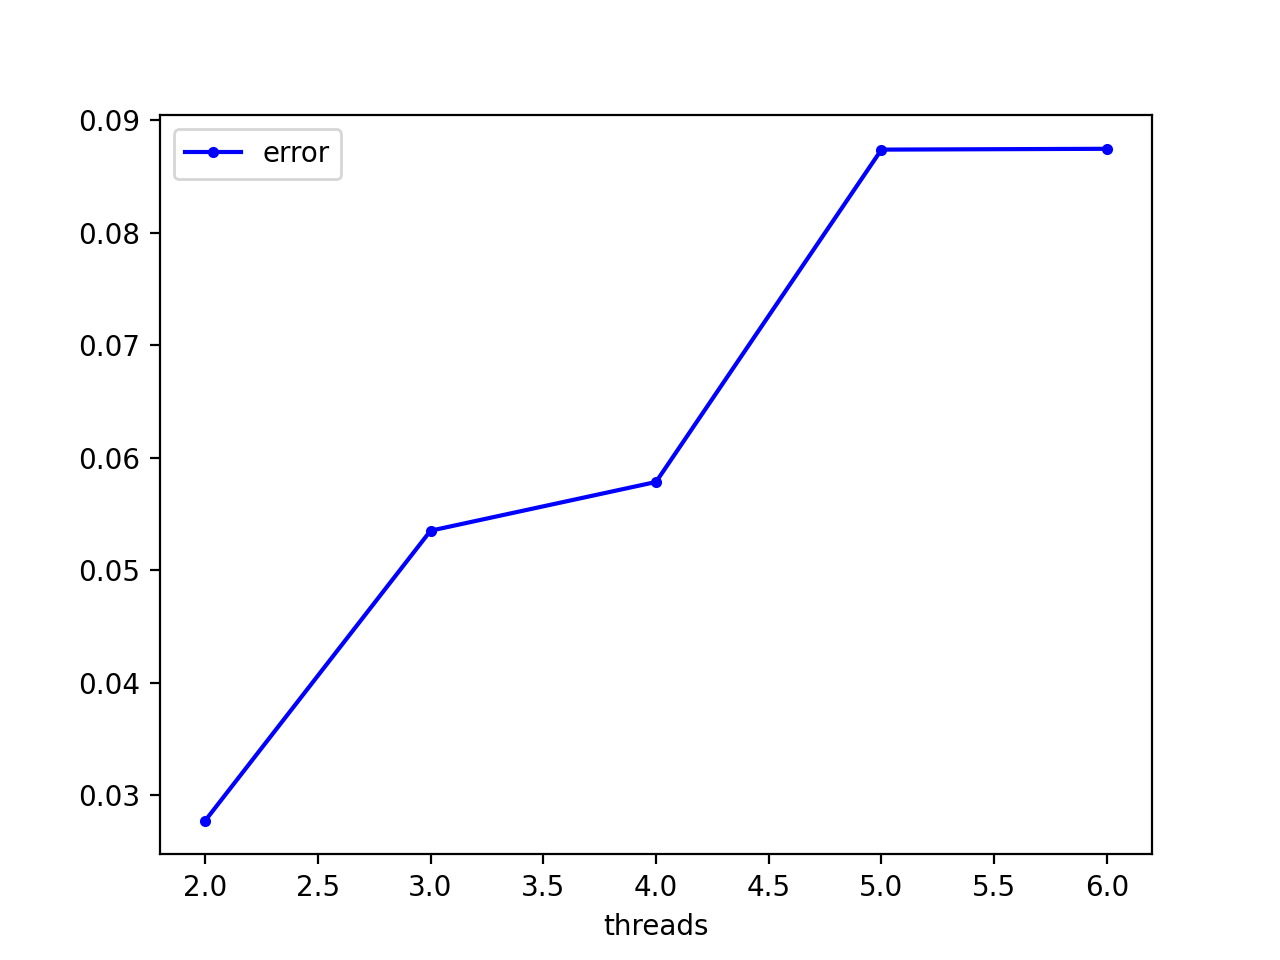
\includegraphics[width=0.5\linewidth]{pthreads-spatial-dynamic-error.png}
    \caption{Error v/s Number of spatial threads}
    \label{fig:pthreads-spatial-dynamic-error.png}
\end{figure}
\begin{figure}[H]
    \centering
    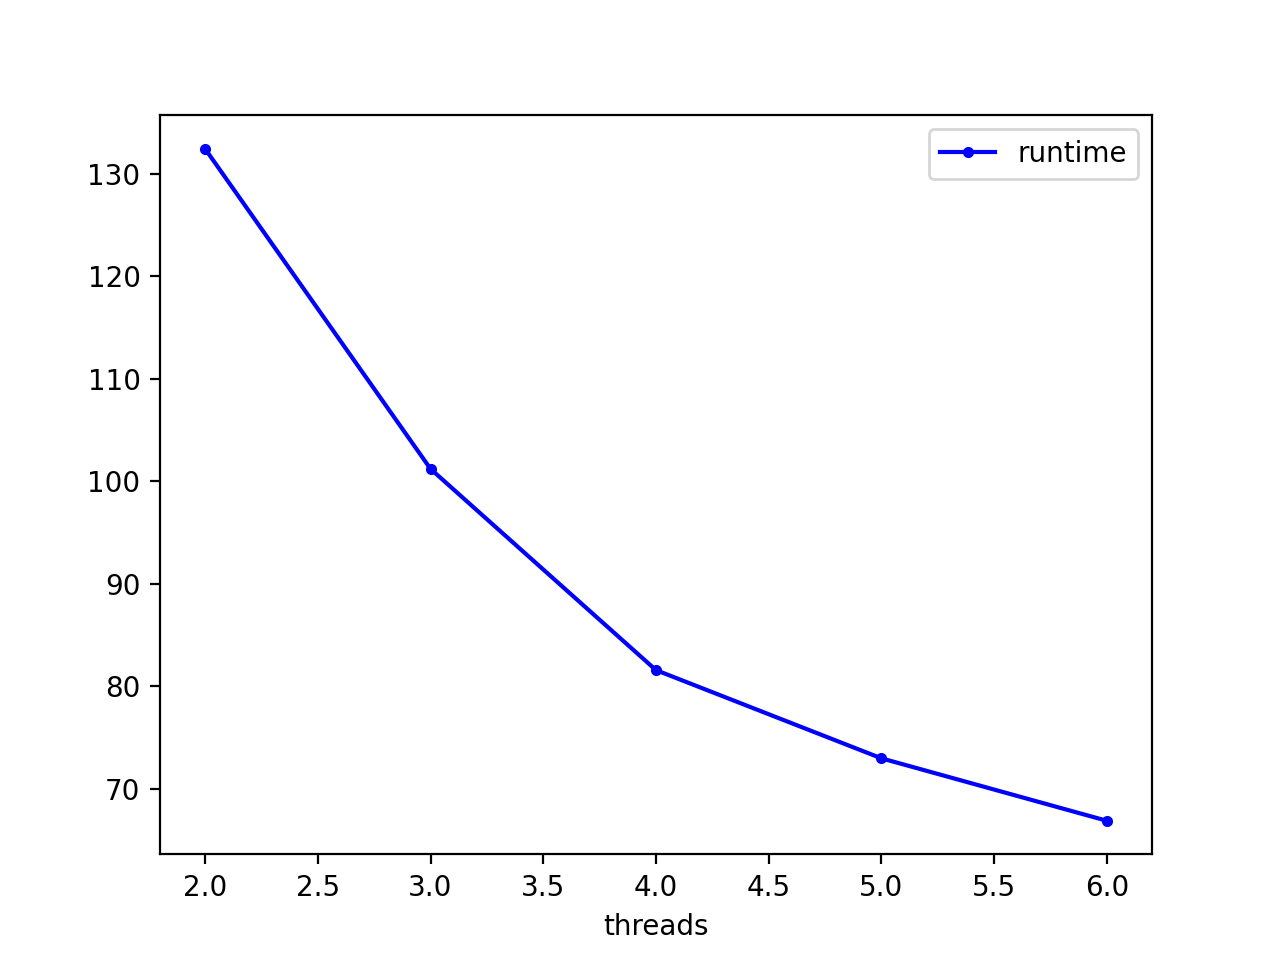
\includegraphics[width=0.5\linewidth]{spatial-pthreads-dynamic-runtime.png}
    \caption{Runtime v/s Number of spatial threads}
    \label{fig:spatial-pthreads-dynamic-runtime.png}
\end{figure}
\begin{figure}[H]
    \centering
    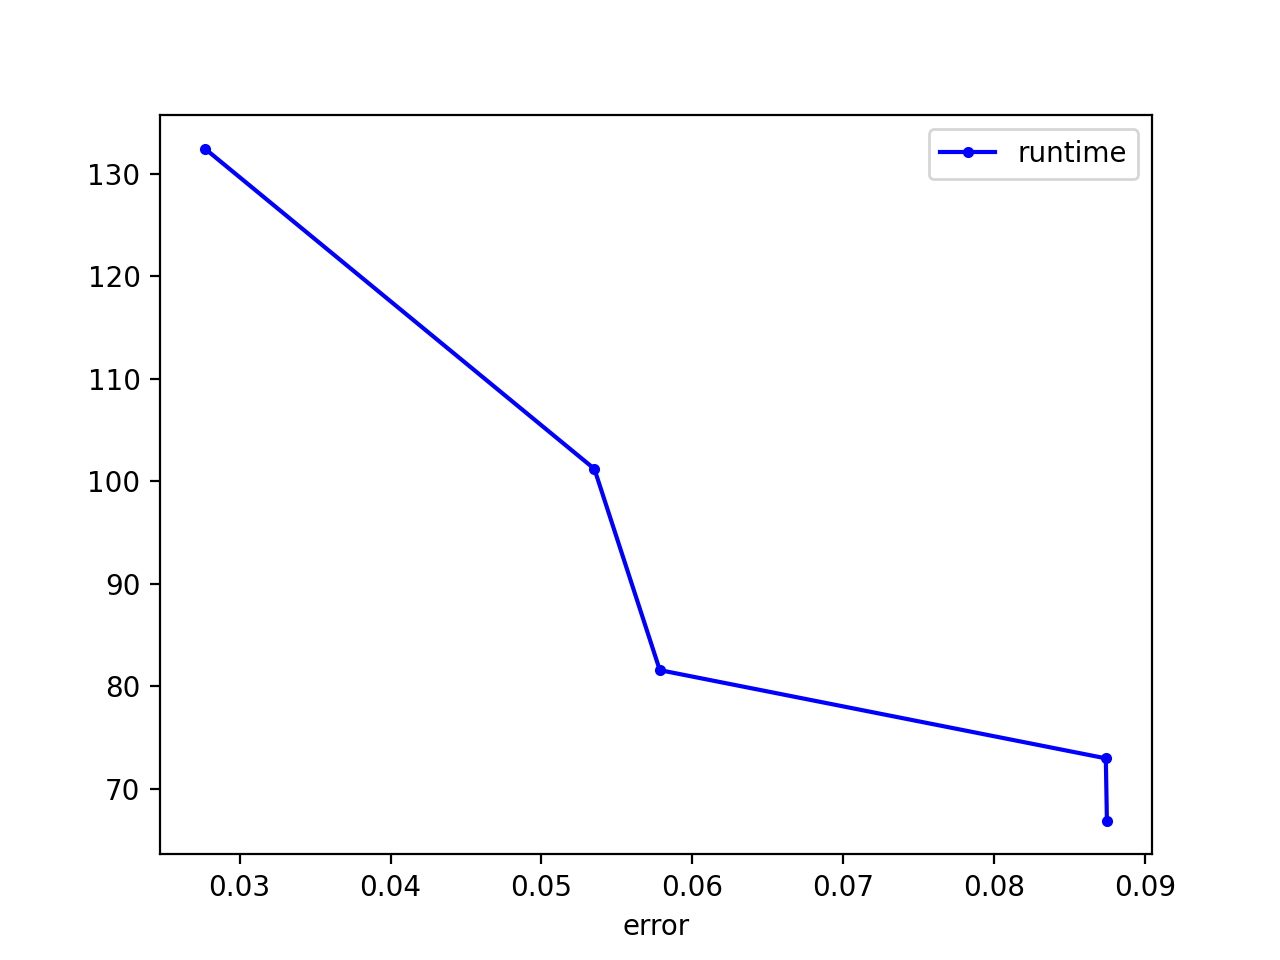
\includegraphics[width=0.5\linewidth]{pthread-spatial-dynamic.png}
    \caption{Error v/s Runtime (in case of spatial threads)}
    \label{fig:pthread-spatial-dynamic.png}
\end{figure}
\begin{figure}[H]
    \centering
    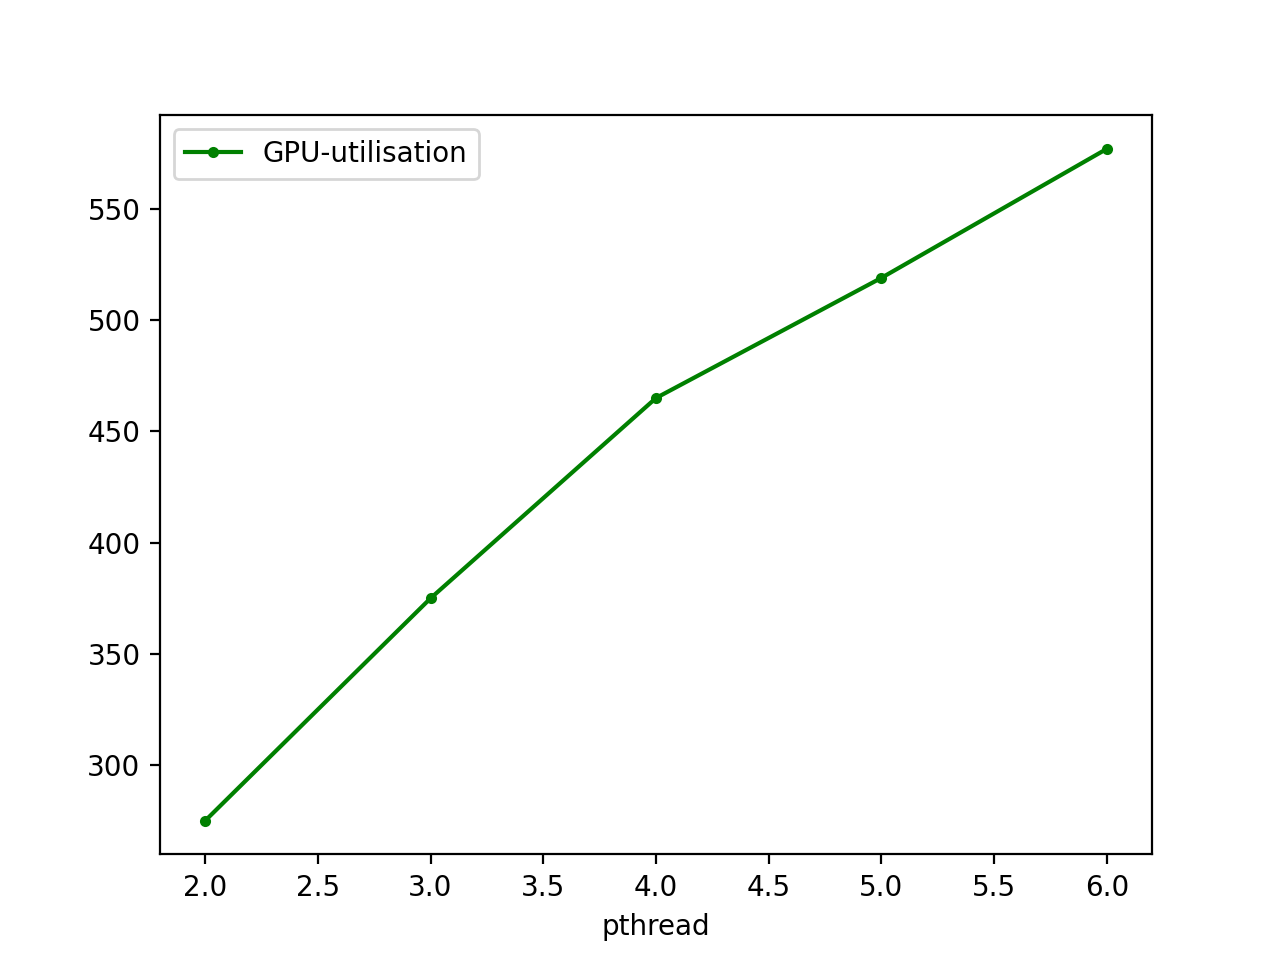
\includegraphics[width=0.5\linewidth]{GPU-spatial-threads-dynamic.png}
    \caption{CPU usage v/s Number of spatial threads}
    \label{fig:pthread-spatial-dynamic.png}
\end{figure}
\begin{figure}[H]
    \centering
    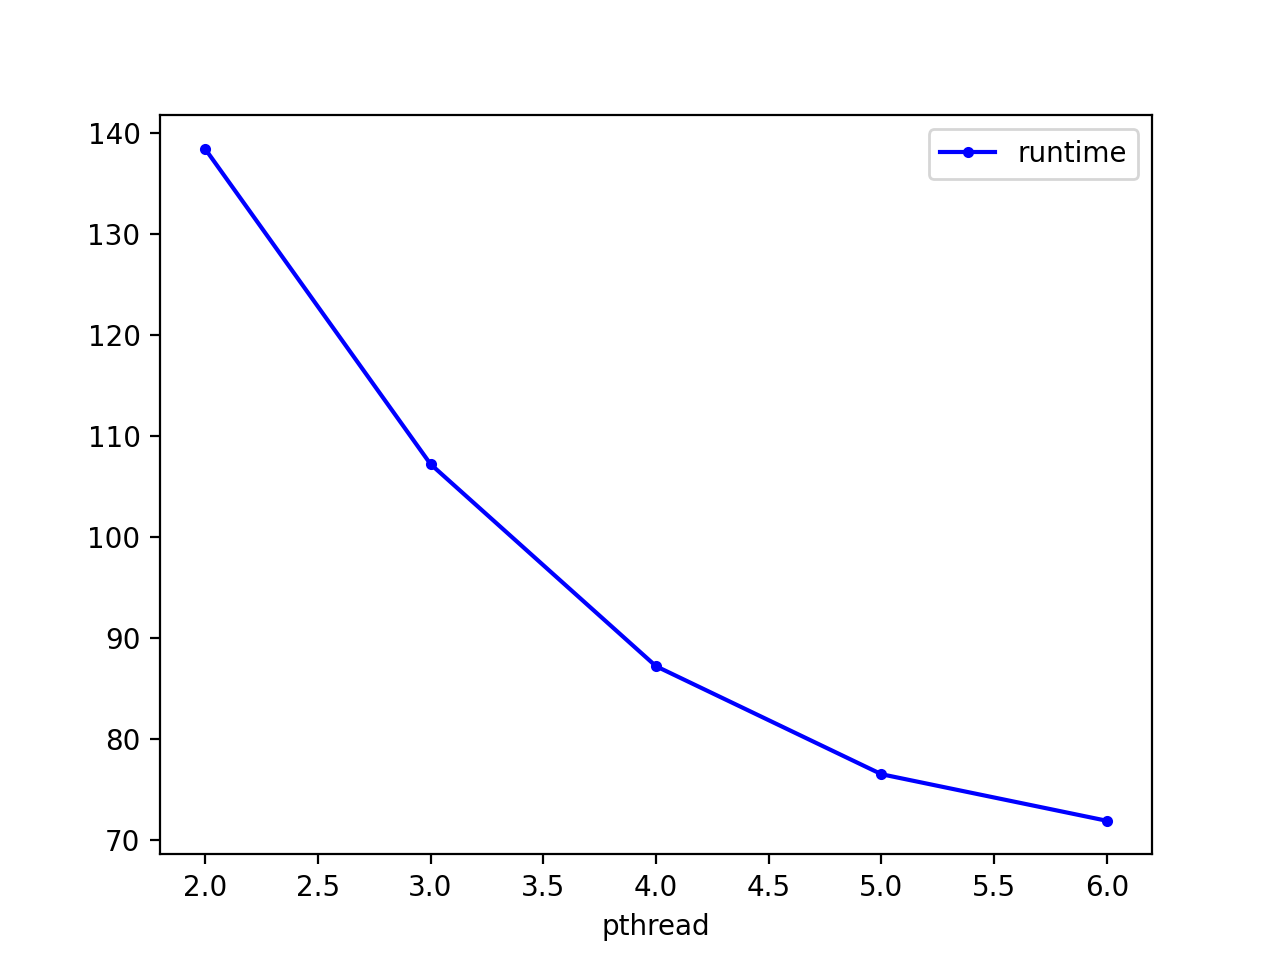
\includegraphics[width=0.5\linewidth]{runtime-temporal-pthread-dynamic.png}
    \caption{Runtime v/s Number of temporal threads}
    \label{fig:pthread-spatial-dynamic.png}
\end{figure}
\begin{figure}[H]
    \centering
    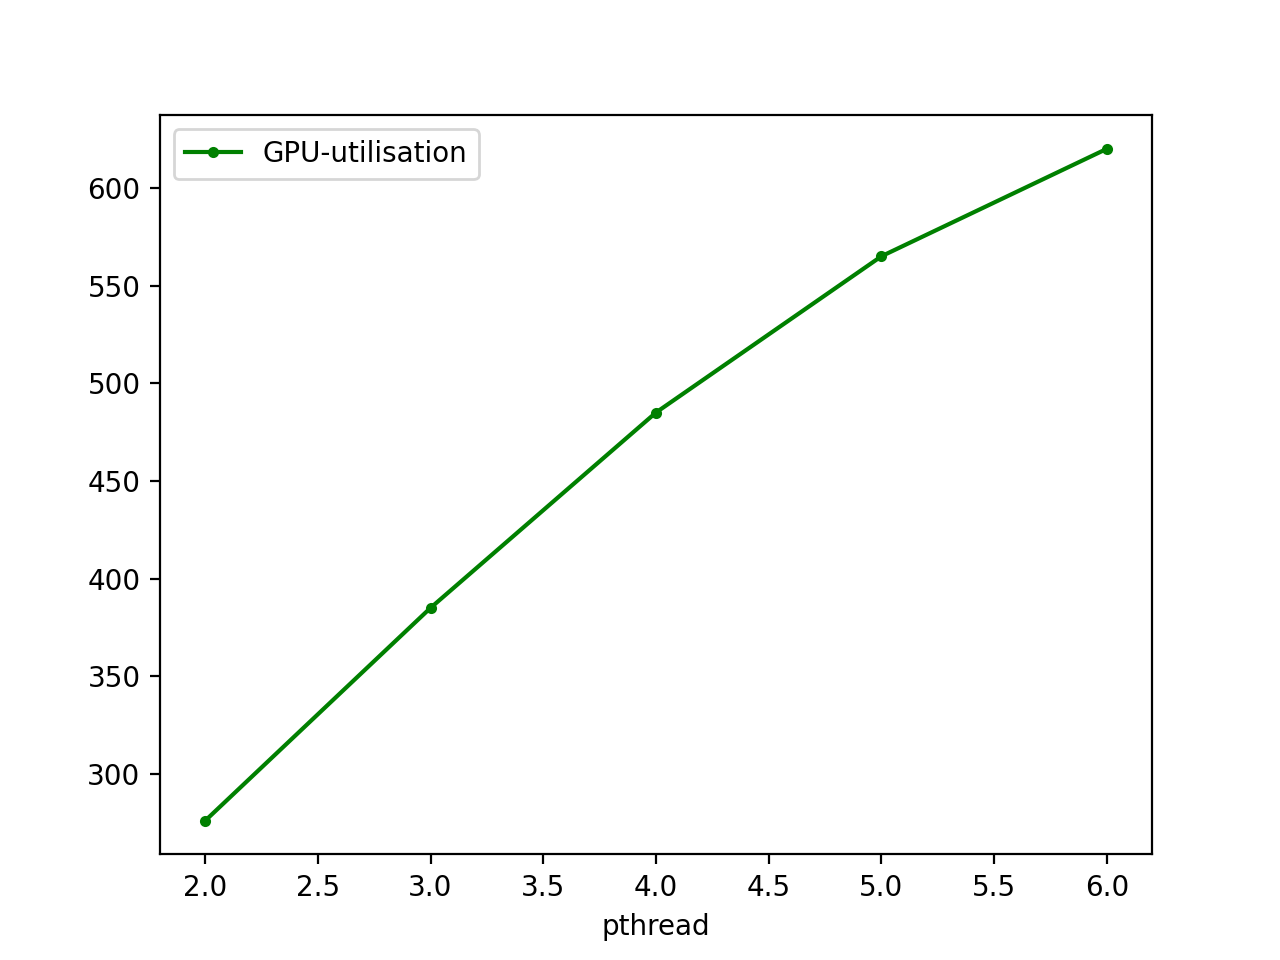
\includegraphics[width=0.5\linewidth]{GPU-utilisation-temporal-pthread-dynamic.png}
    \caption{CPU usage  v/s Number of temporal threads}
    \label{fig:pthread-spatial-dynamic.png}
\end{figure}
%plot of runtime vs utility here 
\subsection*{Observation \& Explanation}
\begin{itemize}
    \item A noticeable runtime v/s utility trade-off is observed in this case. The runtime decreases and the error increases as the number of threads increases.
    \item  This is reasonable since dynamic density estimation is expensive with respect to runtime and dividing its work into threads is likely to reduce runtime substantially.
    \item By Dividing the original frame into several frames, we create several "edges/boundaries" in the image. In the image processing involved in dense optical flow, the edge pixels are not processed as properly as others. Hence the error increases as the number of threads in spatially concurrent dense optical flow increase.
    \item Also, the error in temporal concurrency is negligible in comparison to that in the spatial case which is reasonable since there are no boundary issues in temporal threads, the whole original frame is given to one or the other thread. This shows that temporal concurrency is a better option than the spatial counterpart, given the same number of threads.
    \item The CPU usage increases with increase in the number of threads since more of the resources get allocated to the running program.
\end{itemize}
\section*{Conclusion}
% \subsection*{Methodology}
% \subsection*{Observation \& Explanation}
\begin{itemize}
    \item Method-1,2 , Sparse v/s Dense optical and concurrency in dense optical flow show an obtrusive runtime-utility trade-off.
    \item  However, concurrency seems to gives no advantage in the background subtraction procedure, which is explainable. Concurrency would have led to substantial runtime gains, had the bottleneck procedure for runtime was also parallelized which is not the case with us. Implementing dense optical flow concurrently would have shown the real gains of concurrency. 
    % \item Since sparse flow deals with a smaller set of points, it take lesser time than dense flow.
\end{itemize}
\end{document}

